\chapter{Another Chapter Title}

For a better overview and structured writing, I recommend you place each chapter into a separate .tex file.
As shown in section \ref{text:include-files}, further subdivision of the .tex code is possible if necessary.

\section{Table, Texmaker Keyboard Shortcuts}

For more efficient work with Texmaker, the keyboard shortcuts in table \ref{tab:keyboard-shorts} come in handy.

% Table generated by Excel2LaTeX from sheet 'keyboard-shortcuts'
\begin{table}[htbp]
  \centering

  % \caption{Add caption}
  %% automatic caption created by Excel2Latex is positioned on top of the table
  %% to instead position a caption after the table see below (*)

    \begin{tabular}{ll}
    \toprule
    keyboard shortcut & action triggered \\
    \midrule
    \multicolumn{1}{r}{} & \multicolumn{1}{r}{} \\
    \multicolumn{2}{l}{\textbf{startup procedure}} \\
    Ctrl + Shift + F8 & open files and master from last session \\
    F1    & compile \\
          &  \\
    \multicolumn{2}{l}{\textbf{file navigation}} \\
    Ctrl + F, M & find, find next \\
    Alt + Page Up/Down & switch between open .tex-files \\
    Ctrl + LeftClick in Pdf Viewer & jump to corresponding point in editor \\
          &  \\
    \multicolumn{2}{l}{\textbf{commenting}} \\
    Ctrl + T & comment selected code \\
    Ctrl + U & uncomment selected code \\
    \bottomrule
    \end{tabular}%

	% (*) new caption position below tabular environment, label afterwards!
	\caption{Add caption}
    % within a table, the label has to be called after the caption
    % otherwise there will be a compilation error
	\label{tab:keyboard-shorts}

\end{table}%


The above table is included as a separate .tex file, as described in \ref{text:include-files}.


\section{Packages}

%\usepackage[option1,option2]{package_name}

\section{Error Messages}

This section contains common error messages when compiling .tex into .pdf.
To display possible error messages, activate the window "Messages/Log" within the Texmaker editor as shown in figure \ref{fig:texmaker-messages-log}.

When encountering a new error message, it makes sense to compile once more.
Some errors are caused by incompatibilities between intermediate compilation files and newly written .tex-code. In such a case, recompilation can eliminate those error messages.

\subsection{overfull vbox}

%\lstinputlisting{files/chapters/chapter-2-sections/error-message-overfull-vbox.tex}

%\backslash
"overfull  vbox" means you have too much stuff on a page for LaTeX to arrange nicely. Consider either reducing the size of figures or removing the [H] enforcing the figure to be placed "Here".

%"underfull \vbox" means you have not enough stuff on a page for LaTex to arrange nicely
% consider adding a \pagebreak or \newpage to fill up of extra vertical space

% if "underfull" is the result from a url being too long, add "\hfill" to the corresponding bibtex entry


% TESTING
% Copy the following skeleton report into a standalone .tex file and compile for quick testing

%\documentclass[preview,border=12pt,varwidth]{standalone}
%% \usepackage{optional_package_to_include_inside_the_test}
%
%\begin{document}
%
%test
%
%\end{document}


%
%
%
%\phantomsection \label{def:eps}
%As the permittivity \acs{eps} increases, so does the ability of a given material to attract high voltage breakdown events. \lipsum[3]
%
%
%\section{include sub files}
%
%\input{files/chapters/chapter_2_sections/Molare_Masse}
%
%\section{section name}
%
%\subsection{subsection name}
%
%As shown in chapter \ref{ch:fourty_two}, a subcaption example is still missing:
%
%\begin{figure}
%        \centering
%        \begin{subfigure}[b]{0.3\textwidth}
%                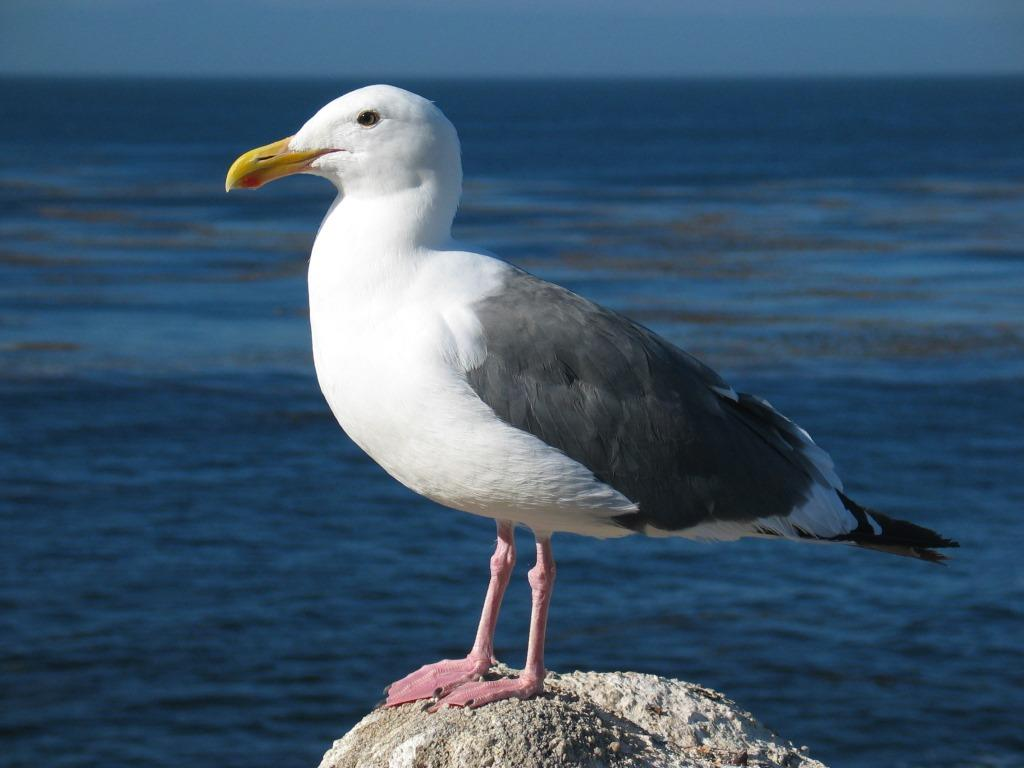
\includegraphics[width=\textwidth]{files/images/gull}
%                \caption{A gull}
%                \label{fig:gull}
%        \end{subfigure}%
%        ~ %add desired spacing between images, e. g. ~, \quad, \qquad, \hfill etc.
%          %(or a blank line to force the subfigure onto a new line)
%        \begin{subfigure}[b]{0.3\textwidth}
%                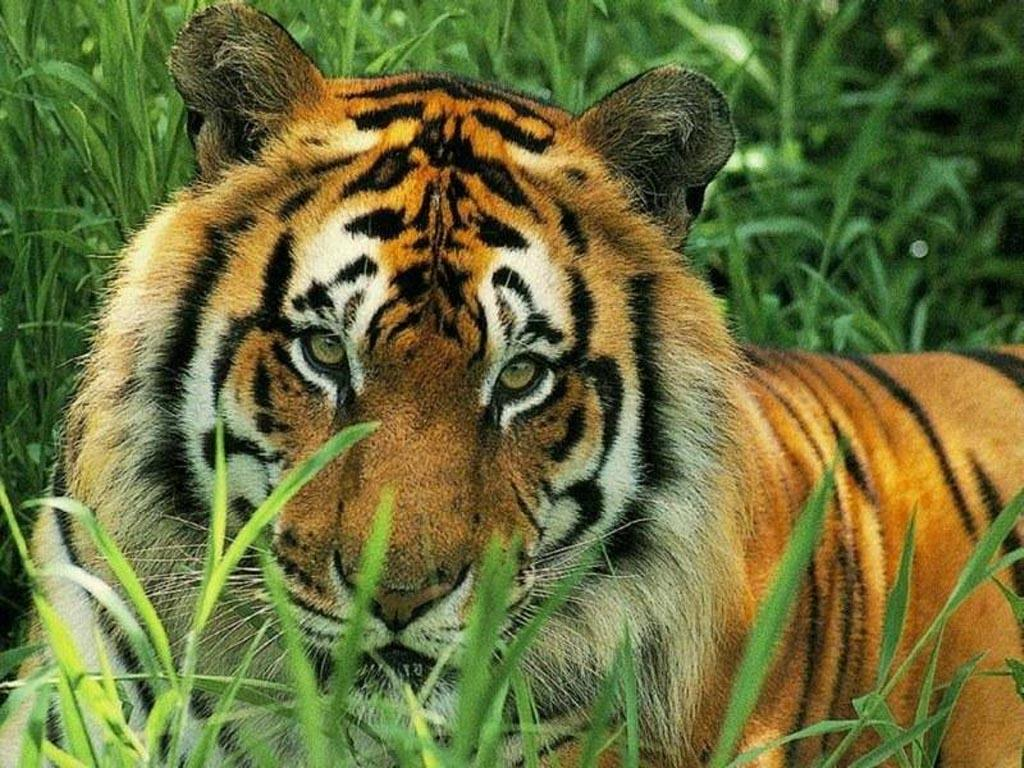
\includegraphics[width=\textwidth]{files/images/tiger}
%                \caption{A tiger}
%                \label{fig:tiger}
%        \end{subfigure}
%        ~ %add desired spacing between images, e. g. ~, \quad, \qquad, \hfill etc.
%          %(or a blank line to force the subfigure onto a new line)
%        \begin{subfigure}[b]{0.3\textwidth}
%                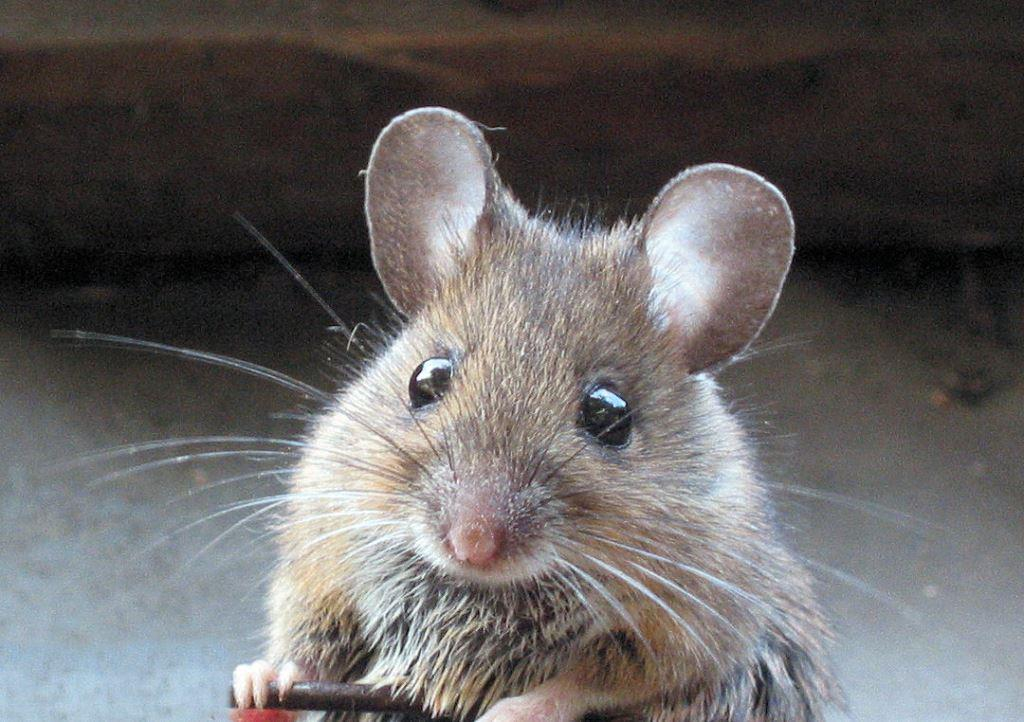
\includegraphics[width=\textwidth]{files/images/mouse}
%                \caption{A mouse}
%                \label{fig:mouse}
%        \end{subfigure}
%        \caption{Pictures of animals}\label{fig:animals}
%\end{figure}
%
%
%
%\subsection{subsection name}
%
%On the other hand, the authors of \cite{2004_Whitesides_writing_a_paper} argue that: \lipsum[4] 

